



%\begin{figure}[!tbp]
%  \centering
%  \begin{minipage}[H]{0.4\textwidth}
%    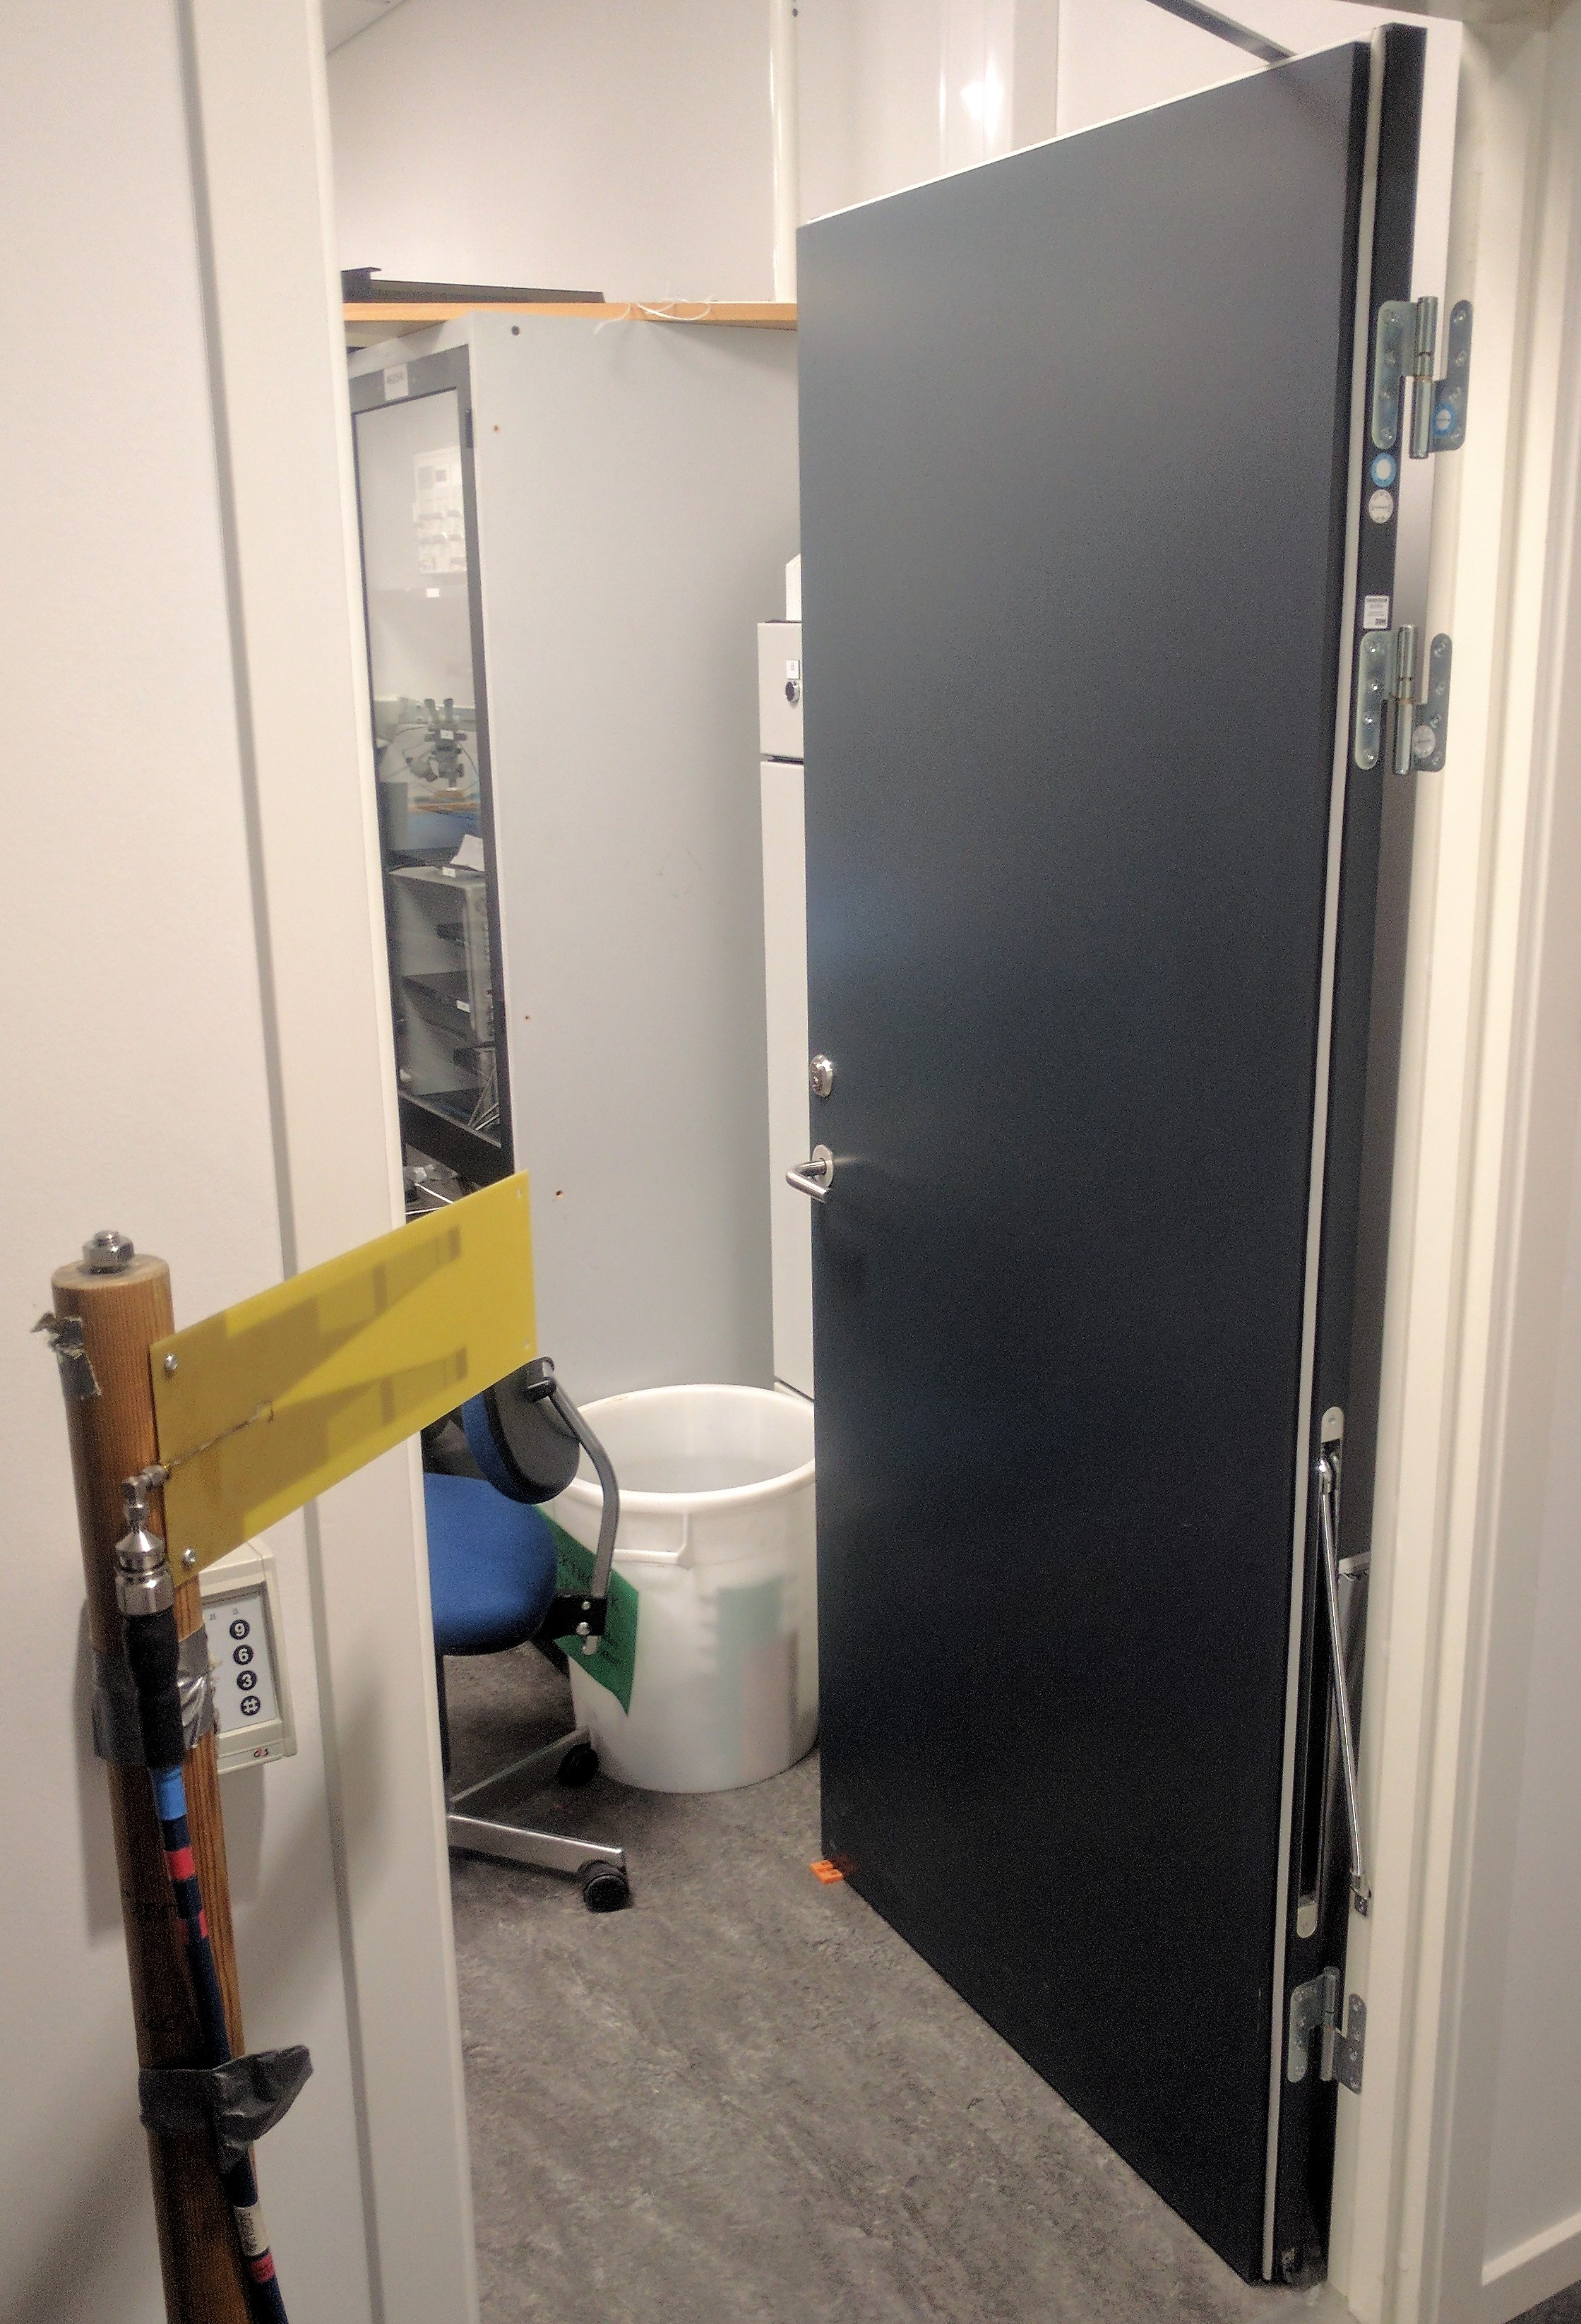
\includegraphics[width=\textwidth]{pictures/Measurement/antenna_door.jpg}
%    \caption{Directional TX antenna.}
%  \end{minipage}
%  \hfill
%  \begin{minipage}[H]{0.1\textwidth}
%    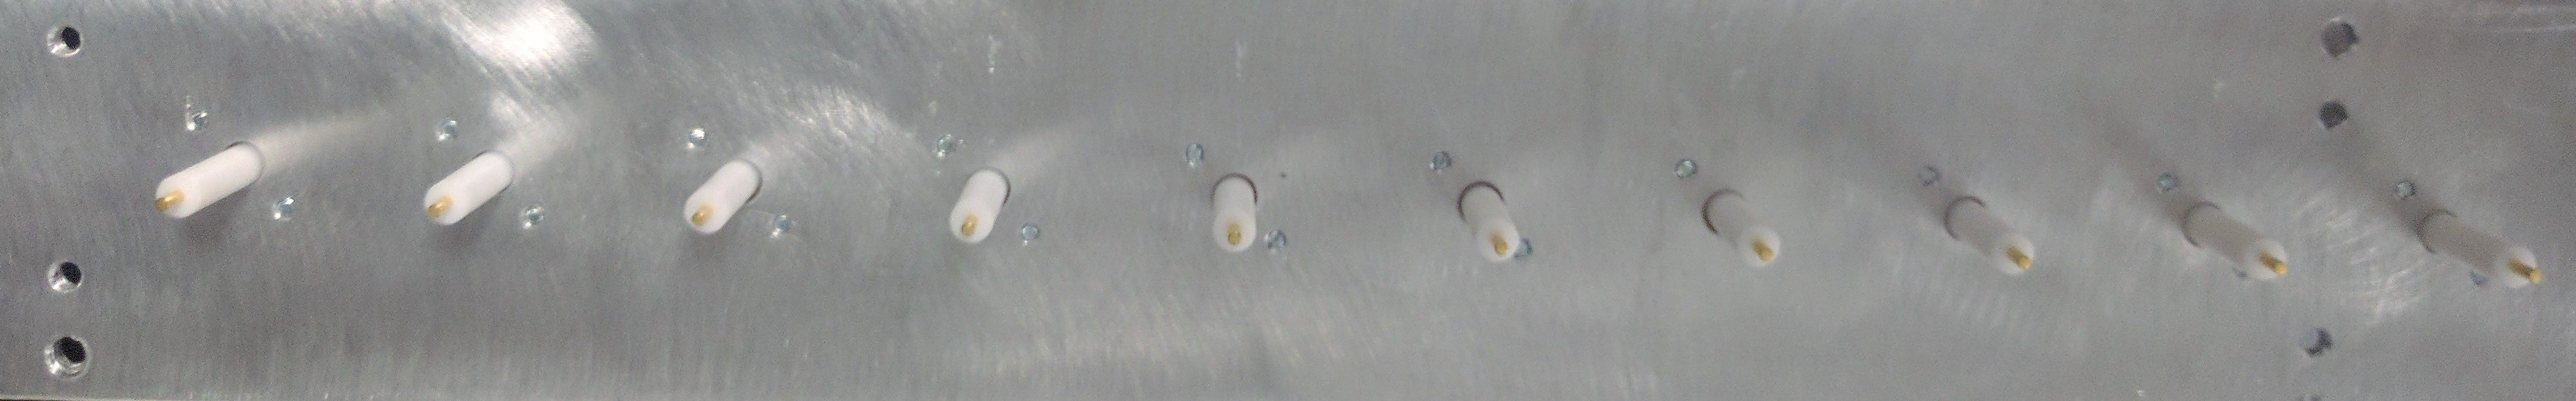
\includegraphics[width=\textwidth]{pictures/Measurement/antenna_array.jpg}
%    \caption{omnidirectional RX antenna array with $\frac{\lambda}{2}$ spacing}
%  \end{minipage}
%\end{figure}



\chapter{Available Resources}
\section{Environment}
The High frequency lab at \gls{AAU} was used for the measurements, it has  clutter and surfaces to give a good representation of a indoor multipath environment. The TX antenna is placed outside of the room pointing towards the door. This provides a NLOS condition. The RX antenna array is moved across the opposite side of the room.

\begin{figure}[H]
  \centering
  \begin{minipage}[H]{0.4\textwidth}
    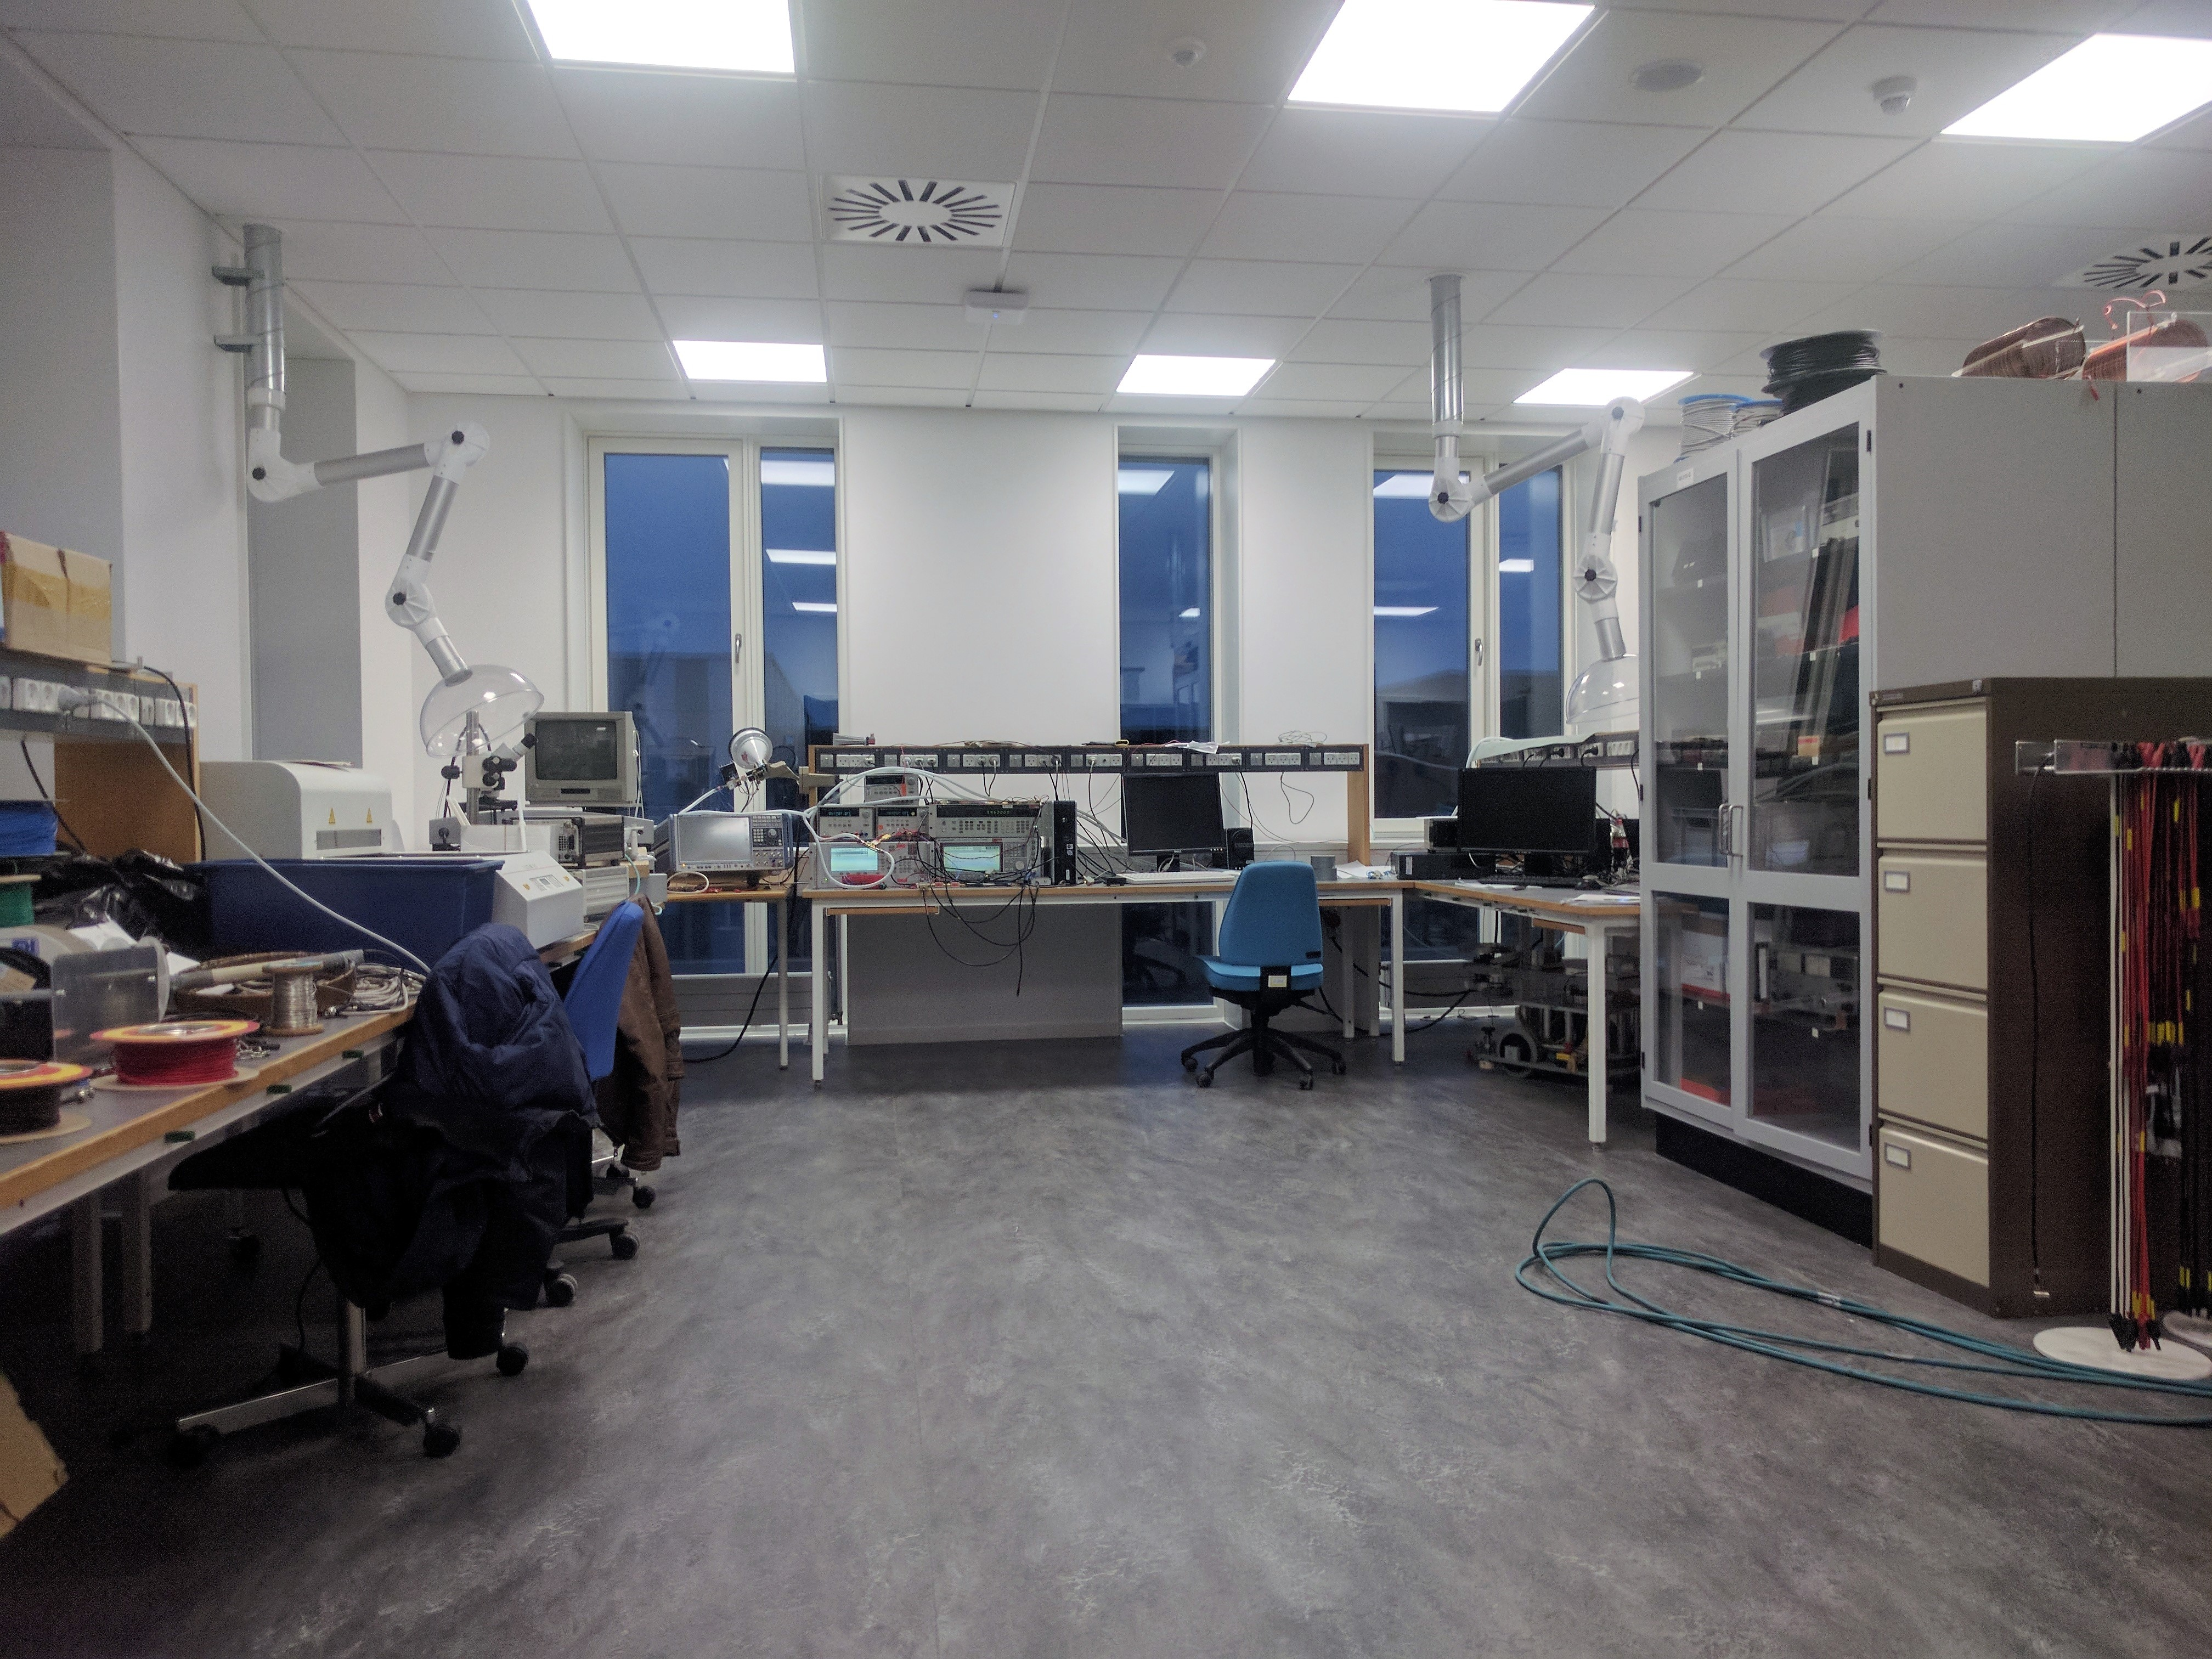
\includegraphics[width=\textwidth]{pictures/Measurement/walking_meas.jpg}
    \caption{Area of the fading gain measurements}
    \label{walk_area}
  \end{minipage}
  \hfill
  \begin{minipage}[H]{0.4\textwidth}
    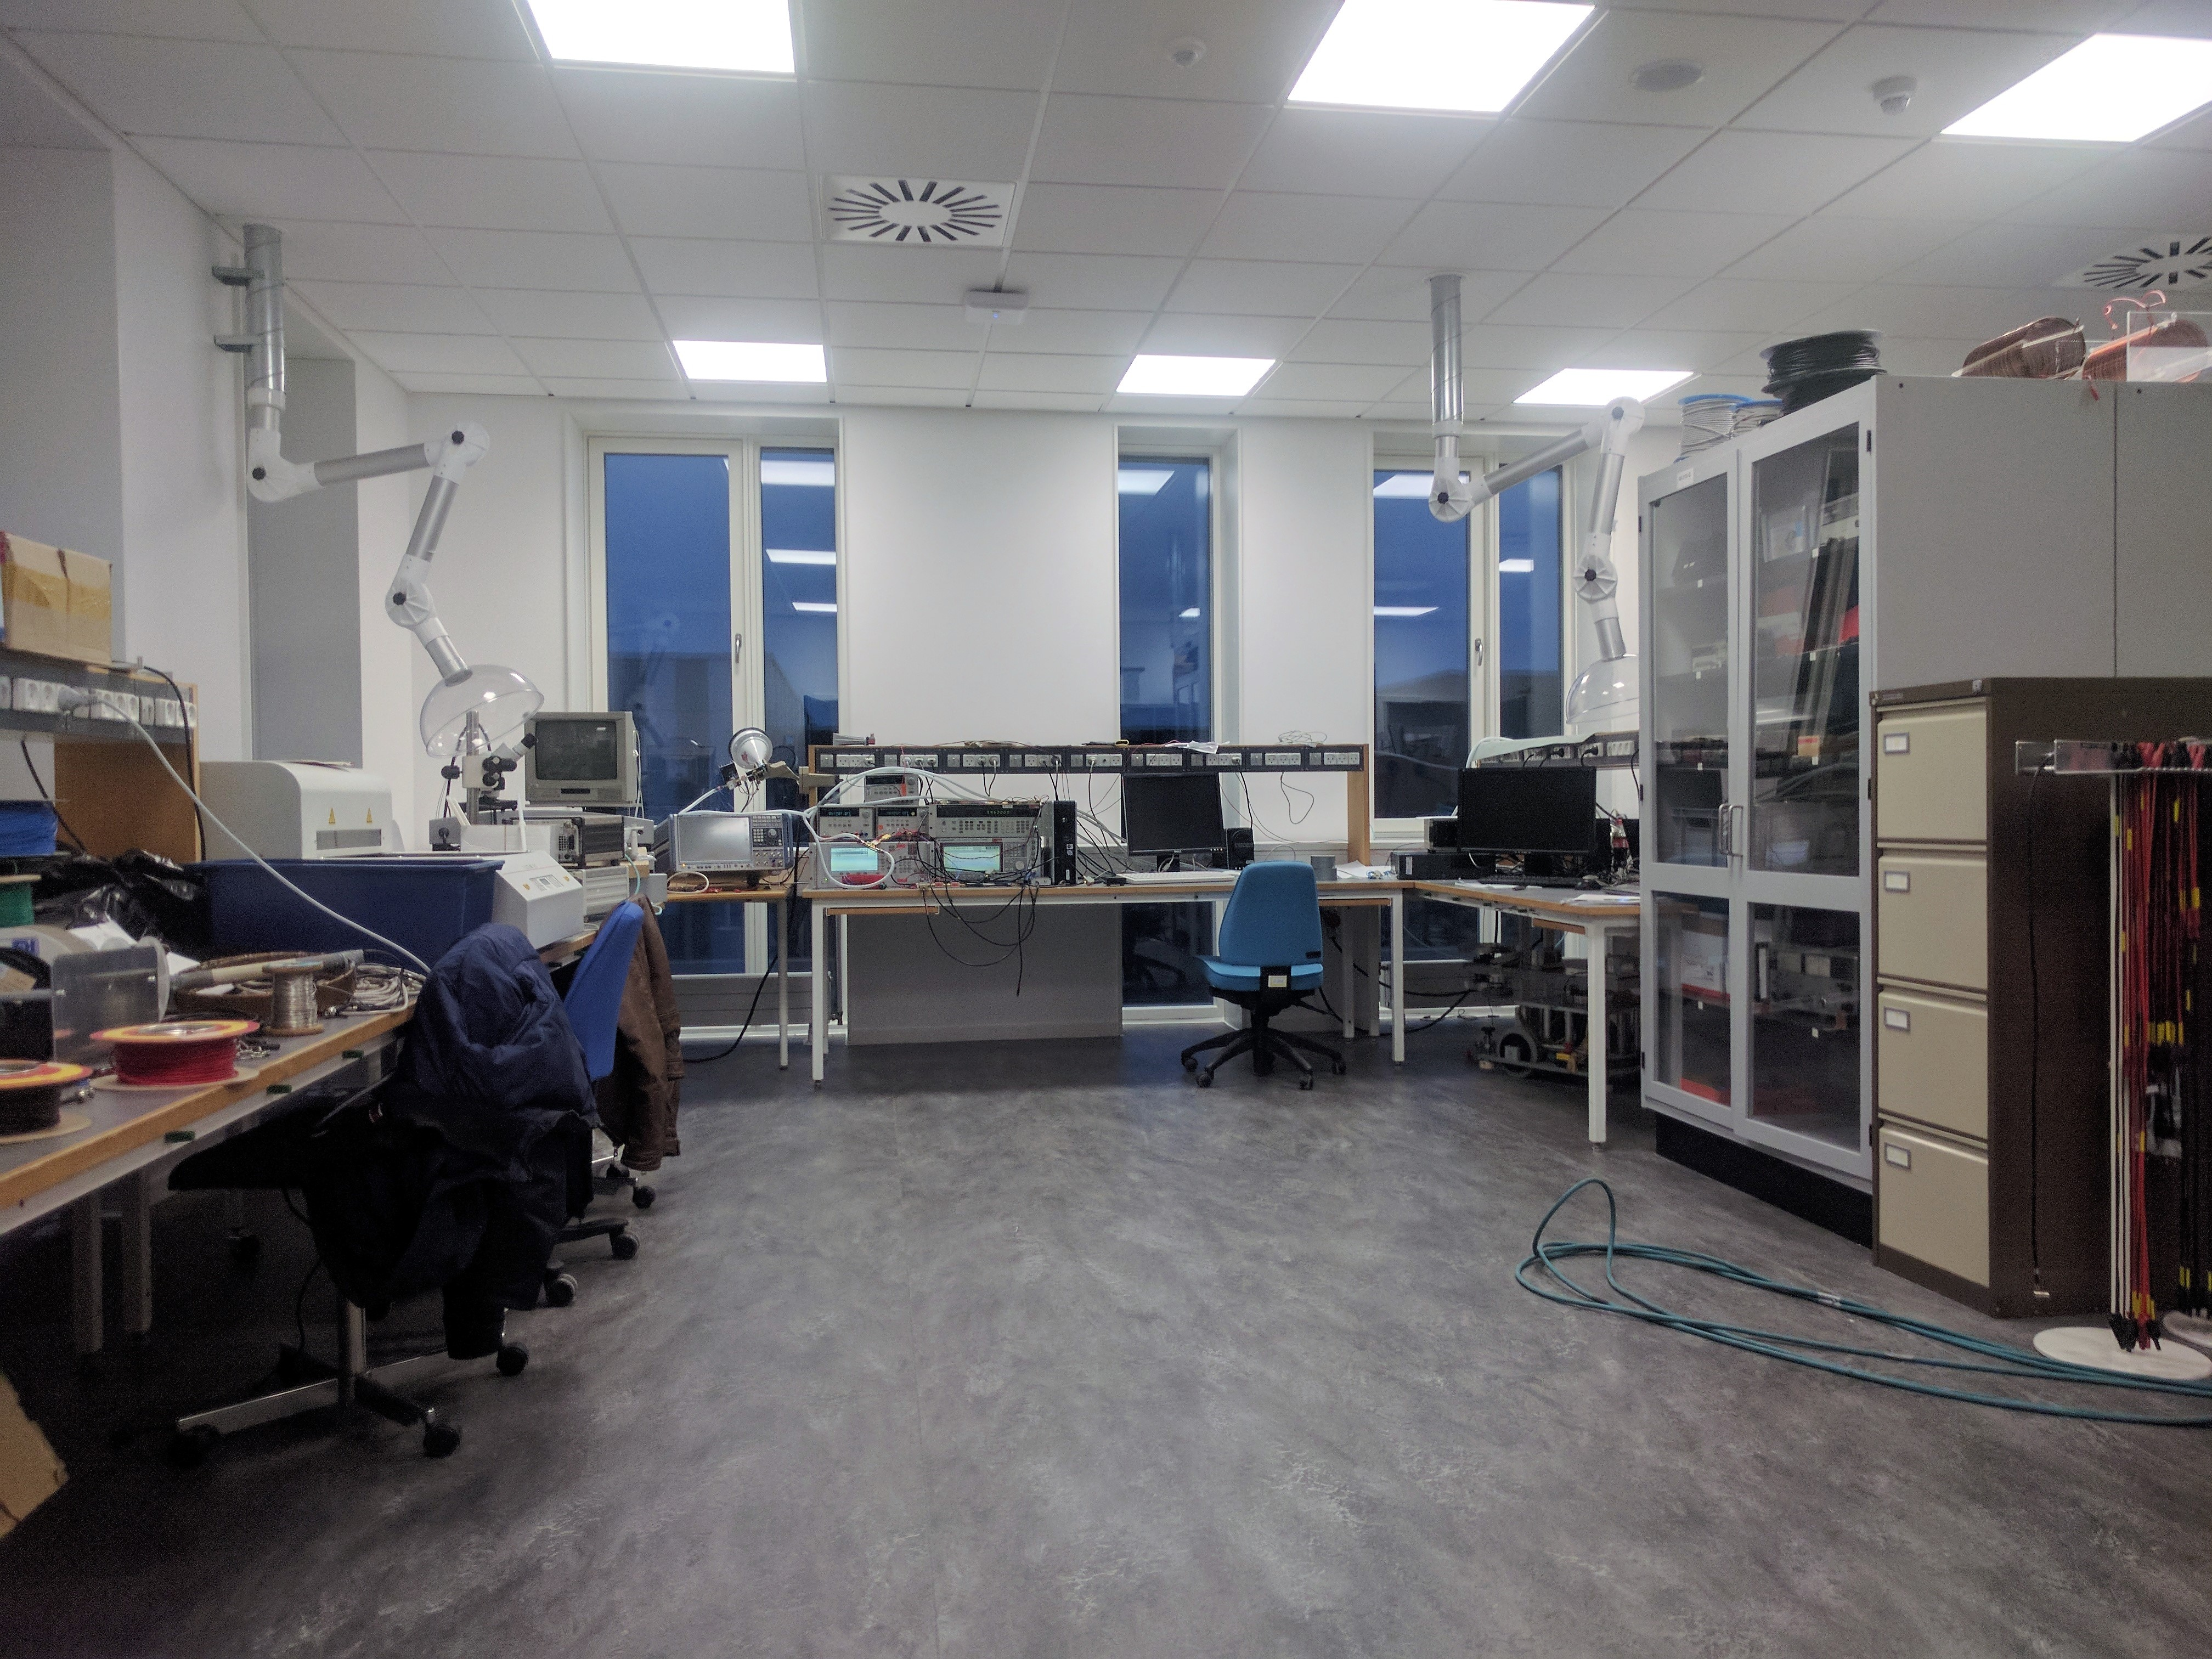
\includegraphics[width=\textwidth]{pictures/Measurement/walking_meas.jpg}
    \caption{Room overview with antenna placement}
  \end{minipage}
\end{figure}
\subsection{Fireplan}

%The setup of the measurement will give the insight and solutions to the problems hypothesised in previous chapters. 
%
%\begin{figure}[H]
%\centering
%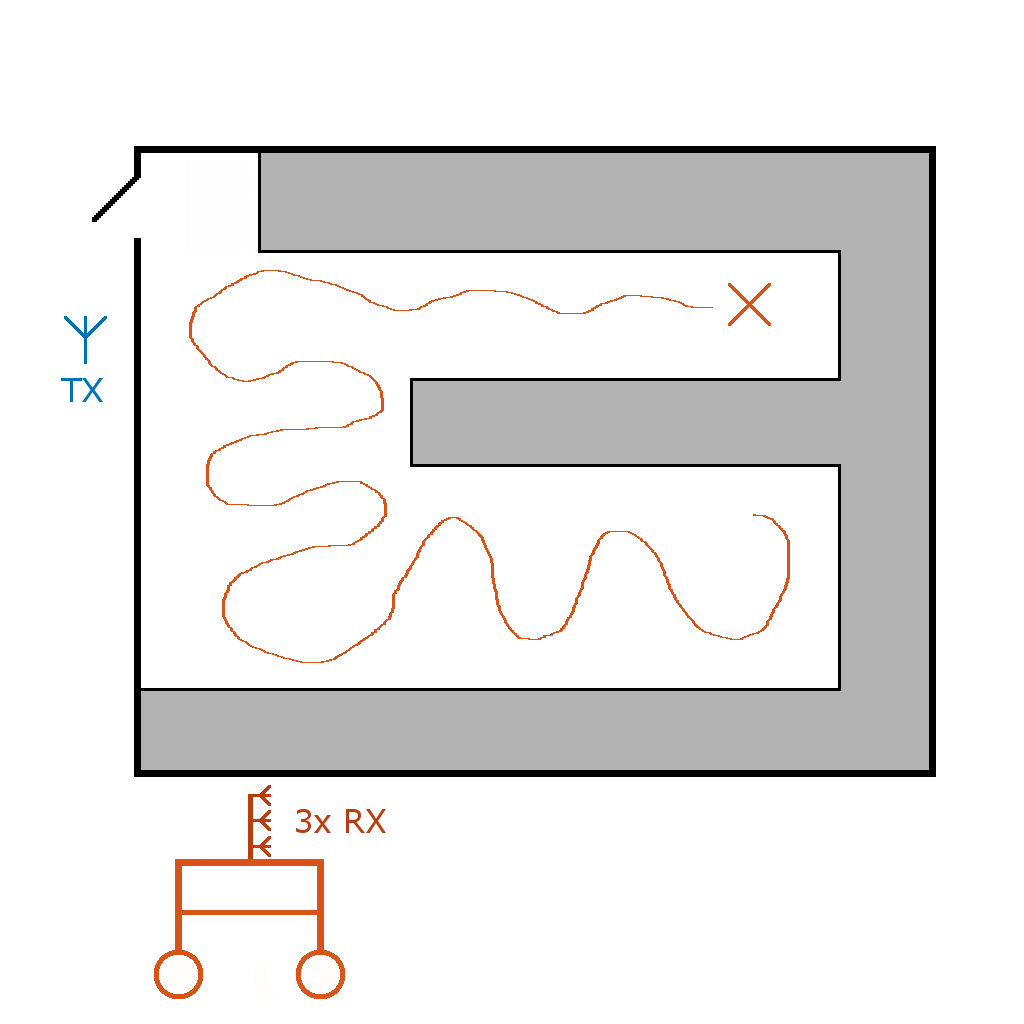
\includegraphics[width=0.75\textwidth]{figures/Gimp_figures/MeasSetup.png}
%\caption{Sketch of the room}
%\label{room sketch}
%\end{figure}
%
%The idea is to do a pilot test of the room. This is to obtain the pathloss $L$ and the delay spread of the room $\sigma_\tau$. With these values we can find the coherence bandwidth $B_c$ and the fading gain can be calculated. 
%We suspect that since this is a multipath NLOS setup the delay spread and pathloss will be very similar across the room. But as a precaution the rooms pathloss and delay will be measured in a close,mid and far region from the doors where the signal originates. When the measurements are ongoing there will be some loss associated with body loss of the handsome scientist and clutter in the environment. This will give more multipath reflections compared to a a empty room.
%\todo {read and rewrite to proper English}
%
%With the pilot test done the full measurement can begin. This will use the same setup as for the pilot test, but with three reviver antennas measuring in parallel and different settings on the VNA. Given the results of the pilot test the amount of samples the sweep will obtain in frequency $N_f$ can be terminated. With this the amount of samples in space can be found to get a total of $4.04 \cdot 10^6$ samples. when the measurement starts the antenna array will be moved slowly in space. During the measurement the operate of the PNA will indicate how fast the person holding the antenna array should walk.



\section{Equipment}
The machine used for the measurement was a Keysight PNA N5527A 4-port VNA with parallel port capture and supports frequencies from 10MHz to 67 GHz.The VNA has a receiver $DR$ of 131dB. With a 4 port VNA the antennas can be set in a 1 TX and 3 RX configuration.This gives antenna diversity of 3. Calibration can be done by connecting the cables together and do a simple normalization. This normalization technique simplifies the calibration, but means a \gls{PA} can't be used.  The sweep data will be saved to a USB.

Cables used have a loss of $0.5dB  \ per \ m$. 3 10m cables and 1 4m cable for the RX and TX antennas respectively. This gives a total cable loss $L_c$ of 7dB.

The TX antenna is a directional antenna with a gain $G_{TX}=12dBi$ at 5GHz.\todo {antenna gain appendix}
The RX antenna array is a omnidirectional antenna with a 5Ghz $f_c$ and a spacing of $>0.4 \lambda$.
\begin{figure}[H]
\centering
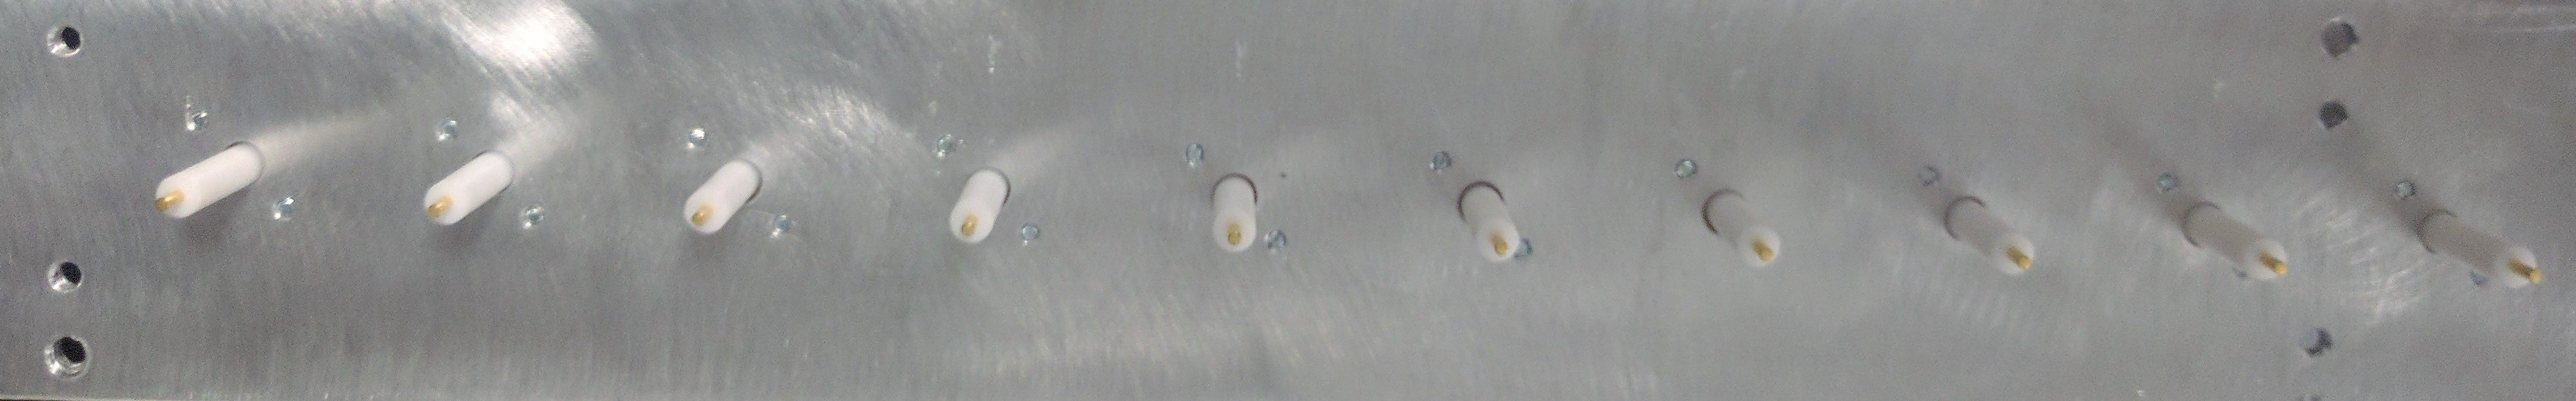
\includegraphics[width=0.7\textwidth]{pictures/Measurement/antenna_array.jpg}
    \caption{Omnidirectional RX antenna array with $0.4 \lambda$ spacing}
\end{figure}
\todo{add a schematic overview of the room}
\begin{figure}[H]
\centering
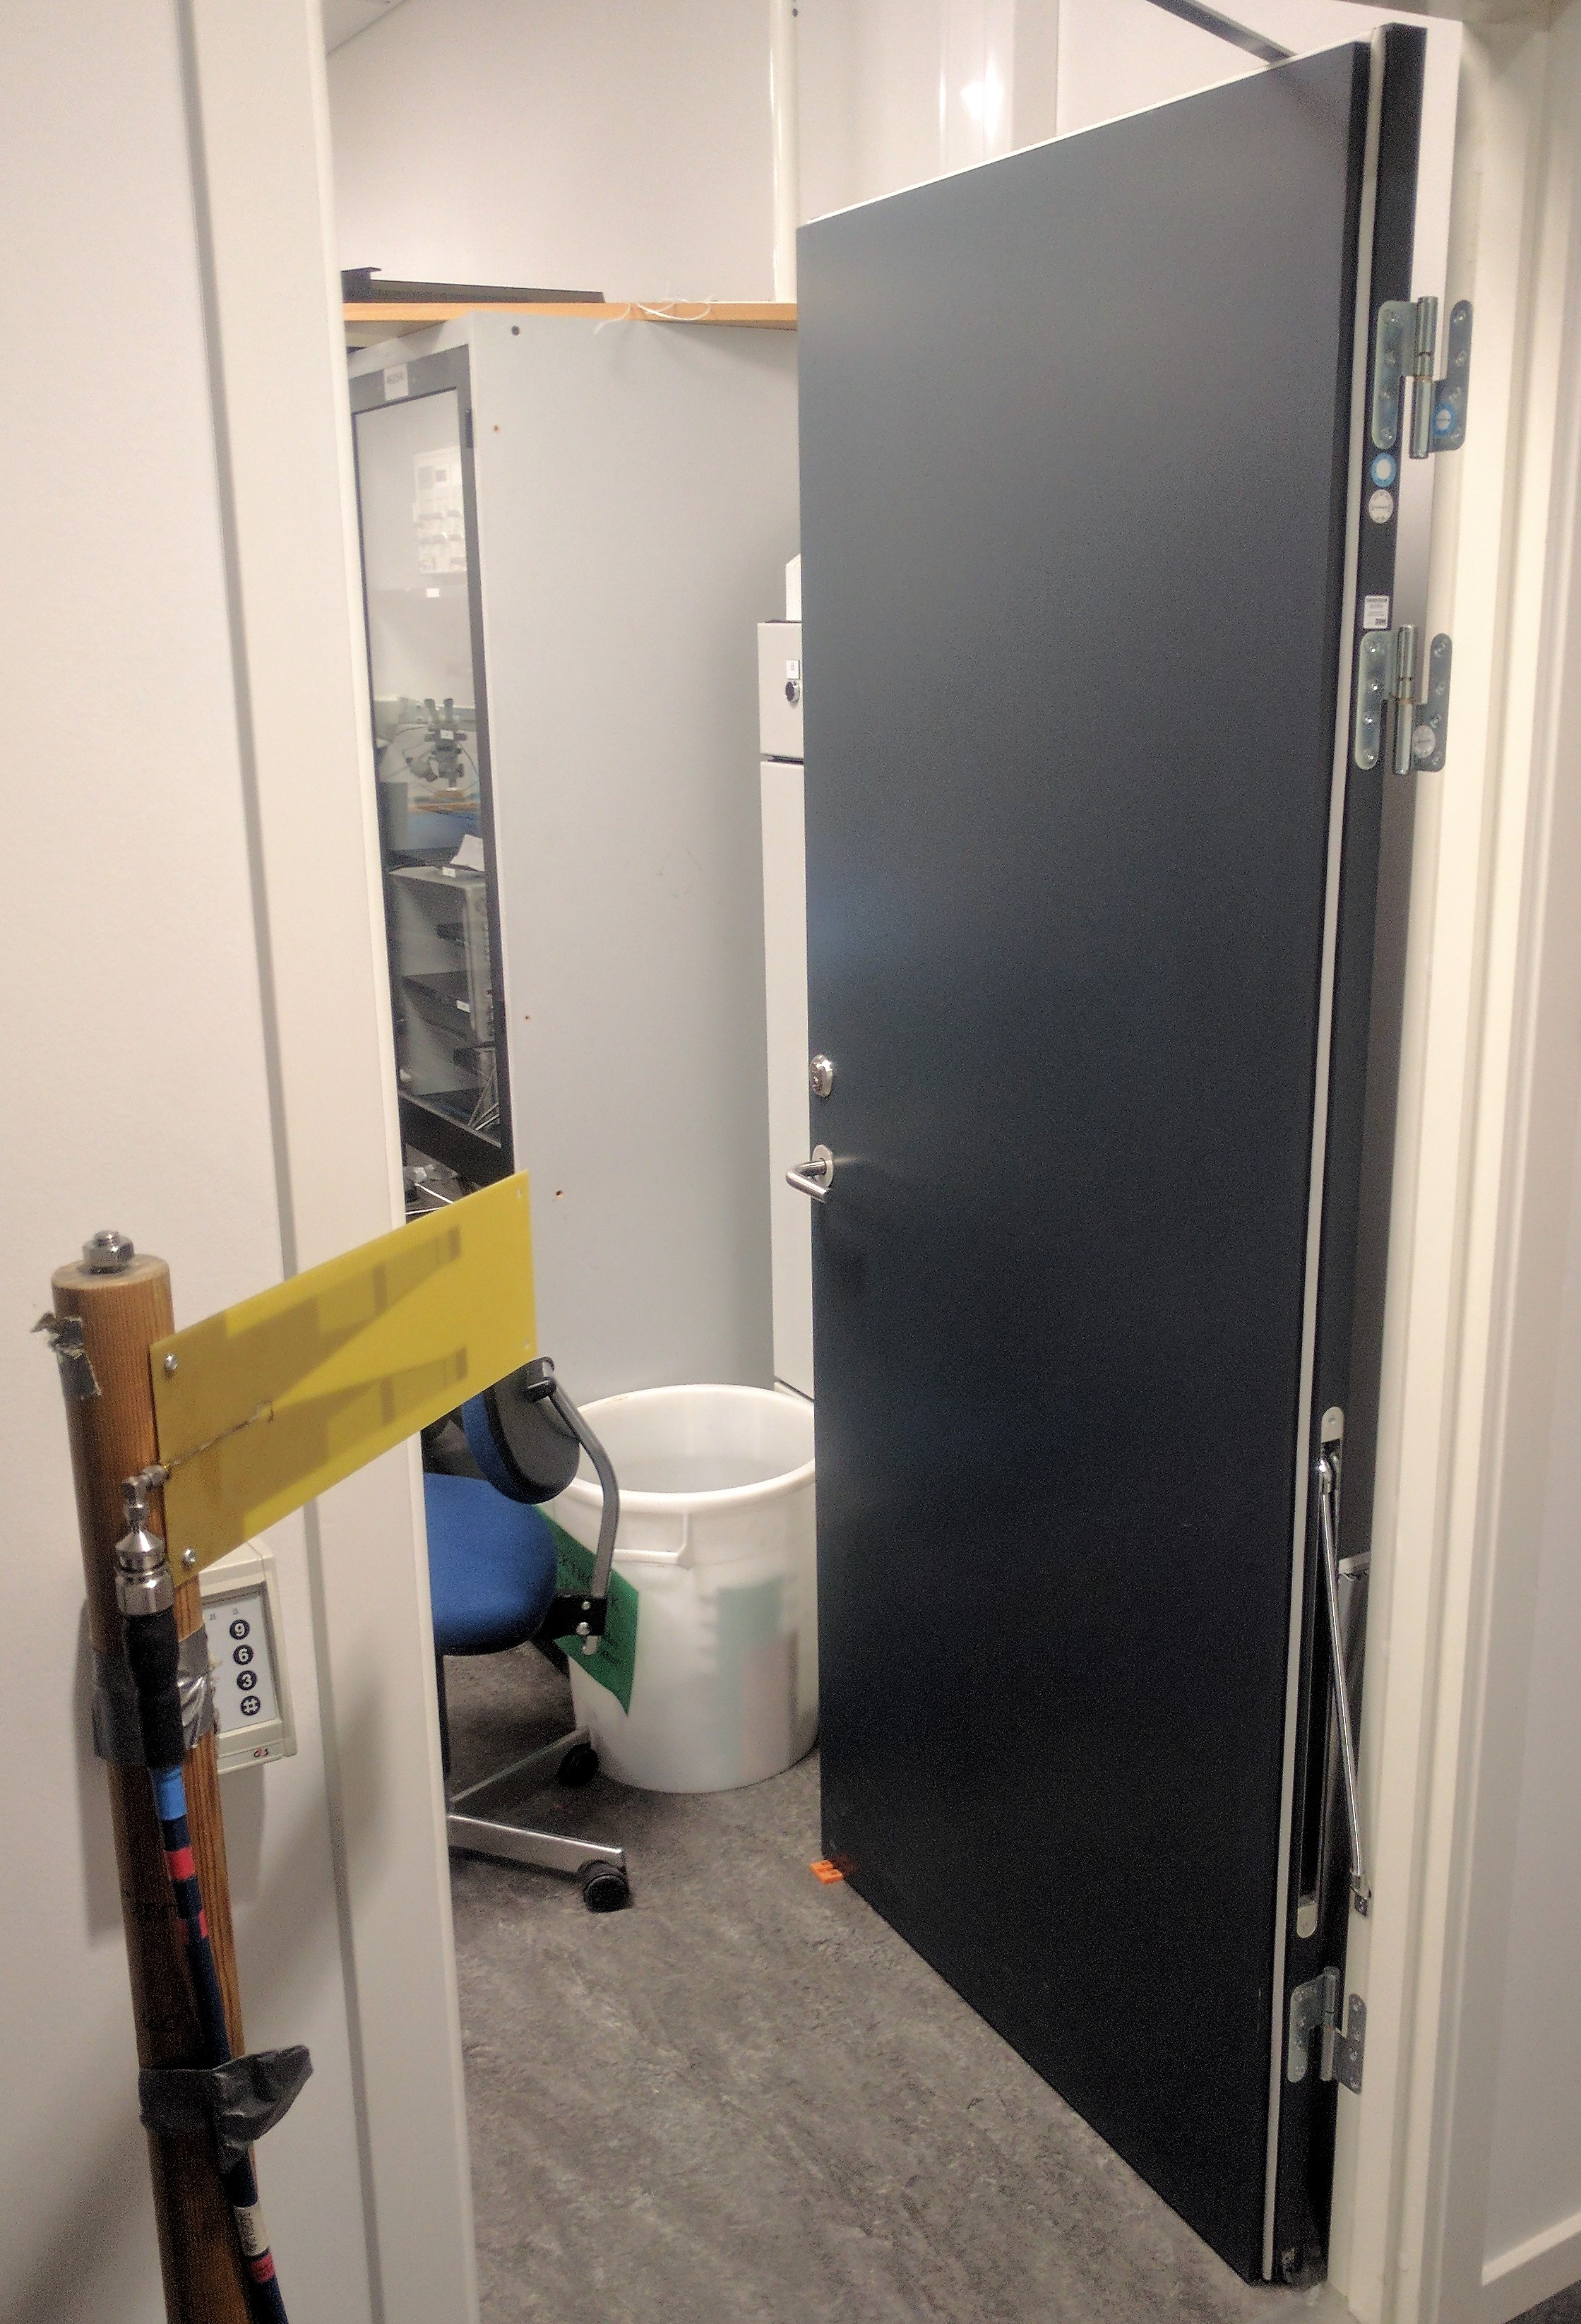
\includegraphics[width=0.4\textwidth]{pictures/Measurement/antenna_door.jpg}
\caption{Directional TX antenna pointing at door.}
\end{figure}


\label{equip}
\subsection{Connected setup}

\begin{figure}[H]
\centering
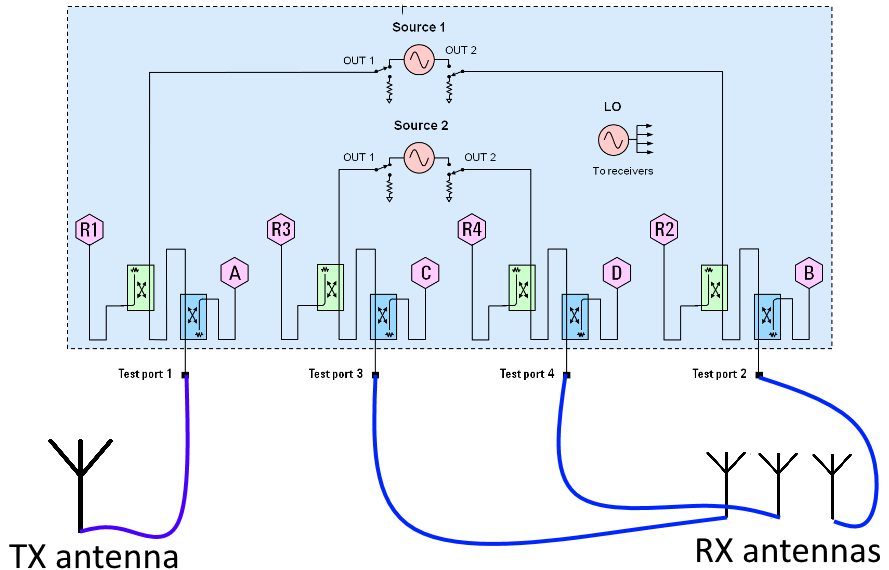
\includegraphics[width=0.65\textwidth]{figures/Gimp_figures/4portVNA.png}
\caption{VNA connections}
\label{connection_diagram}
\end{figure}

The RX antennas was connected directly to the VNA before the coupling (blue box in \autoref{connection_diagram})to reduce the attenuation. After setting up everything we found out that $P_{RX}$ was lower then expected. To increase the $P_{RX}$ the TX antenna was moved closer to the door and a shorter cable was used. The NLOS condition was still fulfilled. 

%Keysight PNA N5527A 4-port VNA with parallel measurements and supports a frequencies from 10MHz to 67 GHz. The sweep data will me saved to a USB.
%
%Cables used have a loss of $0.5dB per m$ 
%Splitter to separate the signal to two TX antennas and point towards the doors for more equal distribution of signal.
%N5527A has a $-119dB$ noise floor without averaging with a 10Hz $IF_{bw}$ at 1-10GHz. The dynamic range of the VNA becomes:
%
%\begin{equation}
%DR = P_{tx}-119dBm 
%\label{NFvna}
%\end{equation}


%The most important part of the setup is the equipment and how they are connected. The R\&S Spectrum Analyser (model FPL9KHz-6GHz) is the center of the setup. This is the receiver of our system and gives us a readout of the spectrum in terms of power (dBm) and frequency (Hz). The two main setting on the Spectrum analyser is IF filter bandwidth and resolution. These two values gives us a sweep time.
\chapter{Setup Parameter estimation}
Before staring measuring the settings on the VNA needs to be determined. This means that the values has to be  balanced to get the needed data and to meet the physical limitations. Part I goes thorough the theory and the limiting factors has been discussed.


\section{TX power}
The transmit power $P_{TX}$ is the maximum power the VNA can transmit without getting overloaded. This should be as high as possible but given that a \gls{PA} is not used this should be around 15dBm \citep{Key_PNA} depending on load from the different antennas and the VNA.
\section{Pathloss}
The ITU pathloss model from \autoref{ITU_model} is used. The planned walking route in the room is around 6 meters from the antenna. This gives a pathloss value of:
\begin{equation}
L = 20log (5000) + 28 \cdot log(6)-28 = 67.76dB \approx 68dB
\label{eq:path_loss}
\end{equation}

The $P_{RX}$ becomes:
\begin{equation}
P_{RX} = 15dBm + 12dBi - 68dB = -41dBm
\label{NFvna}
\end{equation}
\subsection{SNR}
 N5527A has a $-119dB$ noise floor without averaging at 10Hz $IF_{BW}$ between 1-10GHz \citep{Key_PNA}. The \gls{SNR} of the VNA  is defined as:
\begin{equation}
SNR = P_{RX}+W
\end{equation}

\begin{where}
\va{$P_{RX}$}{is the Received power}{dBm}
\va{$W$}{ is the Noise-floor}{dBm}
\end{where}

This gives a SNR of:
\begin{equation}
SNR = -41dBm+119dBm = 78dB
\end{equation}


\section{IF-bandwidth(noise floor)}
Given the $SNR_{M}$ found in \autoref{SNR_margin} and the $SNR$ the diffrence can be used to increese the $IF_{BW}$:
\begin{equation}
  78dB-64dB = 14dB 
\end{equation}

The noise-floor of the \gls{VNA} scales linearly with a increased $IF_{BW}$\citep{PNA_scale}. This means that a $IF_{BW}$ on the \gls{VNA} can be increased to:

\begin{equation}
IF_{BW} = 10Hz \rightarrow 14dB \rightarrow 250Hz
\end{equation}
%\begin{equation}
%\begin{split}
%&= IF_{BW} = -119dB+105dB = 14dB \\
%          \quad &= 10Hz \rightarrow 14dB \rightarrow 250Hz
%\end{split}
%\end{equation}
A higher $IF_{BW}$ of 250Hz  gives a faster sweep time and still meets the requirements set by the $SNR_M$.
\section{FCF}
The delay spread of a signal is very dependant on the environment. For this reason a PDP measurement will measure the delay in the room. Similar indoor values has been measured and shows anything from 20ns delay to 200ns delay for small office environment \citep{indoor_delay}. Since the environment measured fulfills NLOS conditions a $\sigma_{\tau}$ of 50ns is assumed. With the RMS delay spread we can find the approximated $B_C$ which is inversely proportional. 
\begin{equation}
B_C \geq \frac{1}{50ns} \approx 20MHz
\label{CohBW}
\end{equation}
\section{Time estimation}
Since the \gls{VNA} can do segmented sweeps the sweep time is mostly dependant on the number of points and $IF_BW$.
The Keysight PNA N5527A gives the following sweep times for a 201 point with different $IF_{BW}$ \citep{Key_PNA}. \\

\begin{table}[H]
\centering
\caption{$IF_{BW} \ vs \ sweep time$}
\label{my-label}
\begin{tabular}{l|l}
\hline
$IF_{BW}${[}Hz{]} & Sweep time {[}ms{]} \\
10              & 17834               \\
100             & 1825                \\
300             & 641                 \\
1000            & 223                 \\
3000            & 72                 
\end{tabular}
\end{table}

There is also some overhead for saving the data and frequency span. The number of points used in the final setup is dependant $B_C$ and the $\Delta f$. If we use the span of 1GHz and a Coherence bandwidth of 20MHz this gives 50 points. This will reduce the sweep time by quarter.

Let's  use an example where we can use a 300Hz $IF_BW$:
\begin{equation}
T_{sweep \ total} = \frac{631}{4} = 160ms
\end{equation}
This means that every 160ms we have to move $0.4 \lambda$ this gives a relative velocity of:
\begin{equation}
\frac{0.0375m}{0.160s} = 0.23 m/s
\end{equation}
This is under the $1m/s$ value used in \autoref{min_vel}
and total time for moving 5 meters becomes $\approx 22s$.
With the speculated 31200 samples per 5 meter walk(50 samples in frequency and 3 RX antennas) the total number becomes:
\begin{equation}
\frac{4.04 \cdot 10^6}{31200} = 130 \ walks
\end{equation}
or around 48 minuets of continues measurement given 130 walks and 22s per walk. We suspect these values to change depending on the speed at which the data can be saved and the $IF_{BW}$ needed for the desired noisefloor.

\chapter{Measurement of PDP}
\section{setup}
\section{results}
\section{data processing}
\subsection{delay spread}
\subsection{coherence bandwidth}
After the PDP measurements the $B_C$ determined. Together with the $B_C$ and $\Delta f$ the $N_{sweep}$ becomes 41. This will give uncorrelated samples in frequency.

\chapter{Measurement of fading}
\begin{table}[H]
\centering
\caption{Final setting on VNA}
\label{final_specs}
\begin{tabular}{|l|l|l|}
\hline
Number of samples needed         & N           & 4.04 million         \\ \hline
Center Frequency                 & $f_c$       & 5Ghz             \\ \hline
Wavelength                       & $\lambda$   & 6cm           \\ \hline
Coherence Bandwidth                   & $B_C$  & 25MHz           \\ \hline
Span & $\Delta f$ & 1GHz \\ \hline
Dynamic range                    & DR          & XXdB            \\ \hline
Antenna diversity                & $A_{div}$   & 1x3                    \\ \hline
Intermediate frequency bandwidth & $IF_{BW}$     & 500Hz          \\ \hline
Cable loss & $L_{C}$     & 7dB          \\ \hline
Number of points per sweep & $N_{sweep}$ & 41 \\ \hline
Transmit power & $P_{TX}$ & 17dBm \\ \hline
Antenna Gain & $G_{ANT}$ & 12dBi \\ \hline
Sweep time & $T_{sweep}$ &74.1msec \\ \hline
\end{tabular}
\end{table}
   
\section{setup}
The setup was done by moving the antenna array back-and forth in the measurement area in \autoref{walk_area} at three different heights. The toal amount of 5 meter walks done was $3 \cdot 18 = 162$ for a total of 810m.
\section{results}
\section{data processing}
\subsection{stationarity}
K-factor
\subsection{achieved dynamic range}
\subsection{frequency correlation}
\subsection{space correlation}
\subsection{approximate N equivalent}
\subsection{CDF}
confidence values - bootstrap

\section{Results}